\pdfoutput=1 
\RequirePackage{ifpdf} 
\documentclass[12pt,DIV=14,parskip=half]{scrartcl} 

\usepackage{graphicx}
\usepackage{abstract} 
\usepackage[pdftex]{hyperref} 
\hypersetup{
   final,
   a4paper=true,
   pdfpagelayout=TwoPageRight,
   colorlinks=true,
   linkcolor=black,
   citecolor=black,
   filecolor=black,
   bookmarks=true,
   pdffitwindow=true,
   pdfnewwindow=true,
   pdfauthor={ALICE TPC collaboration},
   pdfcreator={pdftex},
   pdfproducer={ALICE TPC collaboration},
   pdftitle={Alice TPC Note},
   pdfsubject={Alice TPC Note},
   pdfkeywords={CERN, LHC, ALICE, TPC} }

\pdfcompresslevel 1 

\title{High-level description of the Digitization of the ALICE TPC with GEM-based readout} 
\author{Andreas Mathis} % (andreas.mathis@ph.tum.de)

\begin{document} 
\maketitle

The work flow of the digitization for the ALICE TPC with GEM-based readout is summarized in Fig. \ref{fig:workflow}.

\begin{figure}
\centering
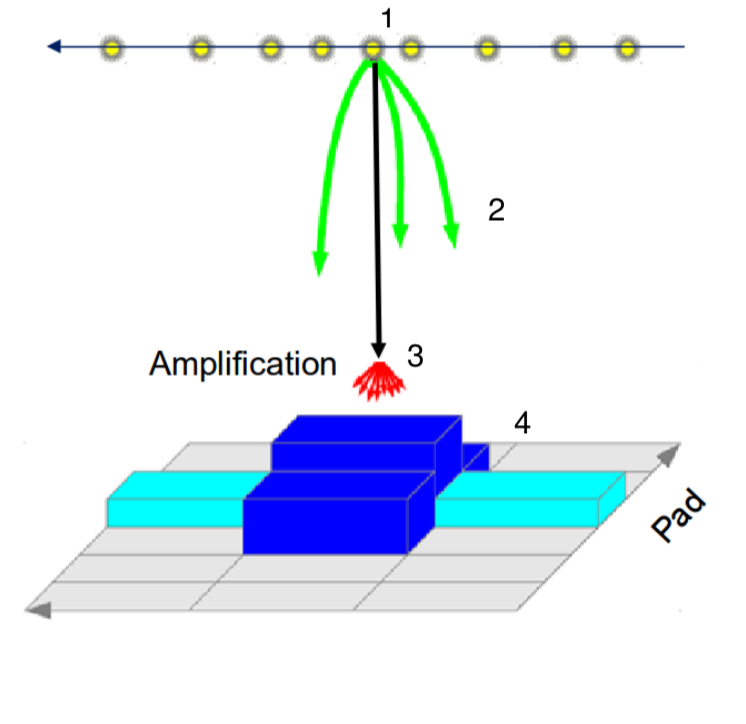
\includegraphics[width=0.6\textwidth]{figures/workflow}
\caption{Summary of work flow and the corresponding physical processes relevant for the digitization in the TPC.}
\label{fig:workflow}
\end{figure}

The digitization starts in DigitizerTask::Exec, where the digit container from previous events is cleared and Digitizer::Process(TClonesArray *GEANT hits) is called.

\begin{enumerate}
\item The energy loss of each individual GEANT hit is converted into a number of electrons by dividing by the effective ionization potential $W_i$ . Each of these electrons is in the following treated individually.

\item The electron is projected onto the readout plane, taking into account diffusion, i.e. smearing its position by a 3D gaussian function (ElectronDrift). Then, the position is transformed into the local coordinate system of the Readout Chamber (ROC).

\item Having arrived at the amplification stage, the electrons undergo successive amplification in each of the four GEM foils (SingleGEMAmplfication), taking into account fluctuations of the gain. These fluctuations follow a Polya distribution.

\item Then, the amplified electrons drift towards the segmented readout anode. The spread of the electron cloud during the amplification stage, as well as the $1/r$ dependency of the Coulomb potential leads to an induction of the signal not only on the pad directly underneath the electron cloud, but also on adjacent pads. The function getPadResponse will return a vector with the coordinates of pads which in this way obtain a signal with respect to the central pad and the weight of the corresponding signal. As this effect is currently not considered, the function just returns $(0, 0, 1)$, which indicated that the central pad receives all the charge.
This charge signal is then folded with the transfer function of the front-end cards (Gamma4) and then successively sorted into the DigitContainer. 
\end{enumerate}

The DigitContainer contains a std::vector with pointers to CRU objects, which in turn contain a std::vector with pointers to Pad Row objects etc. The highest level are the ADC objects, which just contain a single float, as sketched in Fig. \ref{fig:container}.
This makes it very easy to deal with signals stemming from e.g. different tracks, which induce a signal on the same pad in the same time bin. In this situation, the time bin containers would contain two pointers with ADC objects corresponding each to the signal of one track.
When the event is fully processed, DigitContainer::fillOutputContainer( TClonesArray *Digits) is called in DigitizerTask::Exec. Successively, all containers are investigated and, at the highest level, the ADC counts in the ADC objects in one single time bin are summed up. The corresponding ADC value is computed in Digitizer::ADCvalue, taking into account the dynamic range and saturation of the front end cards. 
A pointer to a Digit object is created, which features all the relevant information (CRU, ADC value, pad row, pad, time bin), and is written in the TClonesArray. With this approach, the Digits are sorted according to the CRU, pad row, etc. as required by the cluster finder.

\begin{figure}
\centering
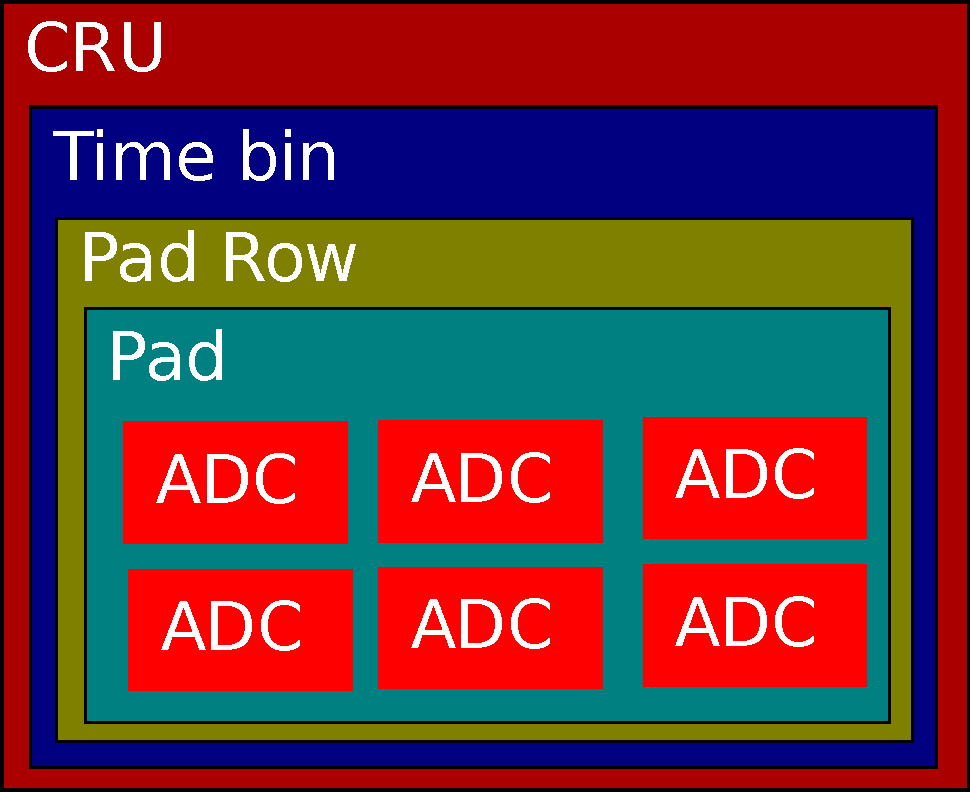
\includegraphics[width=0.6\textwidth]{figures/container}
\caption{Overview of the container in which the digits are stored during digitization.}
\label{fig:container}
\end{figure}

\end{document}